% !TeX program = pdflatex
% =============================================================================
% Zusatzaufgaben: Kondensatoren
% UZH Praktikum I -- Sara Romer Urban, Kantonsschule im Lee, HS2026
% Klassen: 4fh (regulaer, 25.08.2026) + 4cdeg (SP4, 28.08.2026) -- gemeinsames
% Material.
%
% Reine Uebungsaufgaben fuer die Vor-/Nachbereitung (nicht fuer den
% Lektioneneinsatz selbst) -- siehe arbeitsblatt4-kondensatoren-teil1.tex
% (Theorie + Plenum) und aufgabenblatt3-kondensatoren-teil1.tex
% (PhET-/Excel-Lernaufgabe, Partnerarbeit) fuer den Lektioneneinsatz.
% Ursprünglich das einzige Uebungsdokument, per
% Sara Romers Vorgabe (kondensatoren-notizen-sara-romer.txt: "Es soll noch
% ein Aufgabenblatt erstellt werden, welches ein paar Uebungen zum oben
% erwaehnten beinhaltet."); umbenannt zu "Zusatzaufgaben", nachdem der Name
% "Aufgabenblatt" für das neue Partnerarbeit-Dokument gebraucht wurde.
% =============================================================================
\documentclass[addpoints,11pt,a4paper]{exam}

\usepackage[T1]{fontenc}
\usepackage[utf8]{inputenc}
\usepackage[ngerman]{babel}
\usepackage{lmodern}
\usepackage[a4paper,margin=2.2cm,headheight=14pt]{geometry}
\usepackage{amsmath}
\usepackage{siunitx}
\sisetup{per-mode=fraction,fraction-command=\frac}
\usepackage{array,booktabs,tabularx,multirow}
\usepackage{enumitem}
\usepackage{xcolor}
\usepackage{colortbl}
\usepackage{tikz}
\usepackage{physics}
\usepackage{circuitikz}
\usepackage[most]{tcolorbox}
\usepackage{lastpage}
\usepackage{graphicx}

\usetikzlibrary{arrows.meta,calc,angles,quotes}

\usepackage{setspace}
\setlength{\parindent}{0pt}
\setlength{\parskip}{0.6em}
\setstretch{1.08}
\setlist[itemize]{itemsep=0.4em}

% -----------------------------
% Farben (Corporate-Farbschema Physik KFR)
% -----------------------------
\definecolor{titleblue}{HTML}{183A6B}
\definecolor{accentblue}{HTML}{2E6F9E}
\definecolor{lightblue}{HTML}{EAF4FB}
\definecolor{verylightblue}{HTML}{F7FBFE}
\definecolor{lightgray}{HTML}{F4F6F8}
\definecolor{darkgray}{HTML}{4A4A4A}
\definecolor{accentpurple}{HTML}{7B2D8E}
\definecolor{groupteal}{HTML}{1B7F72}
\definecolor{lightgroupteal}{HTML}{E8F5F3}
\definecolor{lightpurple}{HTML}{F3EAF7}

\newcolumntype{Y}{>{\centering\arraybackslash}X}
\newcolumntype{P}[1]{>{\raggedright\arraybackslash}p{#1}}

\tcbset{before skip=10pt, after skip=10pt}
\newtcolorbox{titlebox}{
  enhanced, colback=titleblue, colframe=titleblue, boxrule=0pt, arc=3mm,
  left=3mm,right=3mm,top=3mm,bottom=3mm
}

\newlength{\aufgabenindent}
\settowidth{\aufgabenindent}{10.\hskip\labelsep}

% Praktikum I: Lernziele/Einleitung/Theorie/Aufgaben werden NICHT mehr
% farbig gerahmt (nur Formel-, Hinweis- und Antwortbox bleiben Boxen) --
% siehe institutionen/UZH-Praktikum-I/CLAUDE.md, Abschnitt "Boxen-Layout".
\newenvironment{infobox}{%
  \par\addvspace{10pt}\noindent
}{%
  \par\addvspace{10pt}
}

% taskbox/groupbox stehen in questions VOR dem ersten \question (Bilder,
% Fliesstext) -- exam.cls' questions-Liste braucht dafür eine echte,
% eigenständige Box (sonst "Something's wrong--perhaps a missing \item",
% weil z.B. ein \begin{center} vor dem ersten \item der Aussenliste steht).
% Deshalb bleiben es tcolorboxen, nur unsichtbar gemacht (keine Farbe/Rahmen,
% kein Padding) statt sie durch reine Absätze zu ersetzen.
\newtcolorbox{taskbox}[1][]{
  enhanced, breakable,
  colback=white, colframe=white, boxrule=0pt,
  left=0mm,right=0mm,top=0mm,bottom=0mm,
  before skip=10pt, after skip=10pt,
  before upper={%
    \def\tmpboxtitle{#1}%
    \ifx\tmpboxtitle\empty\else\noindent\textbf{#1}\par\smallskip\fi
  }
}

\newtcolorbox{groupbox}[1][Gruppenarbeit]{
  enhanced, breakable,
  colback=white, colframe=white, boxrule=0pt,
  left=0mm,right=0mm,top=0mm,bottom=0mm,
  before skip=10pt, after skip=10pt,
  before upper={\noindent\textbf{#1}\par\smallskip}
}

% formelbox: kurze Formelsammlung zum Nachschlagen -- kein Theorie-Ersatz,
% keine Herleitung (siehe arbeitsblatt4-kondensatoren-teil1.tex dafür), nur
% die fertigen Formeln als Gedächtnisstütze für die Vor-/Nachbereitung.
\newtcolorbox{formelbox}[1][Formel]{
  enhanced, breakable, colback=lightpurple, colframe=accentpurple,
  title={#1}, fonttitle=\bfseries, boxrule=0.9pt, arc=2mm,
  left=5mm,right=5mm,top=2mm,bottom=2mm
}

\newtcolorbox{answerbox}{
  breakable, colback=white, colframe=gray!55, boxrule=0.5pt, arc=1.5mm,
  left=2mm,right=2mm,top=2mm,bottom=2mm
}

% --- Lösungen ein-/ausblenden -----------------------------------------------
\noprintanswers
%\printanswers

\pointformat{}
\renewcommand{\solutiontitle}{\noindent\color{titleblue}\textbf{Lösung:}\enspace}

\pagestyle{headandfoot}
\cfoot{\textcolor{darkgray}{Seite \thepage\ von \pageref{LastPage}}}

\newcommand{\Kopfzeile}[4]{%
  \begin{titlebox}
    {\color{white}\sffamily\bfseries\Large #4}
  \end{titlebox}
  \vspace{0.5em}
  \noindent\textbf{Klasse:}~#1 \hfill \textbf{Datum:}~#2 \hfill \textbf{Thema:}~#3
    \hfill \textbf{Lehrperson:}~Loris Keller
  \vspace{0.8em}
  \lhead{\textcolor{darkgray}{#3}}
  \rhead{\textcolor{darkgray}{#4}}
}

\newlength{\antwortraumlen}
\newcommand{\Antwortraum}[1]{%
  \pgfmathsetlength{\antwortraumlen}{#1*2.5cm}%
  \begin{answerbox}
    \rule{0pt}{\antwortraumlen}%
  \end{answerbox}%
}

\newcommand{\Klasse}{4fh / 4cdeg (SP4)}
\newcommand{\Datum}{25.08.2026 (4fh) / 28.08.2026 (4cdeg)}
\newcommand{\Thema}{Kondensatoren}
\newcommand{\ZusatzaufgabenTitel}{Zusatzaufgaben: Kondensatoren}

\begin{document}

\Kopfzeile{\Klasse}{\Datum}{\Thema}{\ZusatzaufgabenTitel}

\begin{infobox}
\textbf{Zu diesen Zusatzaufgaben}\\
Diese Übungsaufgaben ergänzen das Arbeitsblatt und das Aufgabenblatt
\emph{Kondensatoren} und sind für die Vor-/Nachbereitung gedacht, nicht für
den Lektioneneinsatz selbst. Alle benötigten Formeln und Herleitungen
findest du im Arbeitsblatt.
\end{infobox}

\begin{formelbox}[Formelsammlung]
\[
  Q = C\cdot U, \qquad C = \varepsilon_0\cdot\frac{A}{d} \quad\text{(ohne Dielektrikum)}, \qquad C = \varepsilon_r\cdot\varepsilon_0\cdot\frac{A}{d} \quad\text{(mit Dielektrikum)}.
\]
$\varepsilon_0\approx\SI{8.85e-12}{\farad\per\meter}$; $Q$ in \si{\coulomb};
$U$ in \si{\volt}; $C$ in \si{\farad}; $A$ in \si{\meter\squared}; $d$ in
\si{\meter}; $\varepsilon_r$ dimensionslos ($\varepsilon_r>1$).
\end{formelbox}

\begin{questions}

\begin{taskbox}[Aufgabe 1: Kondensatorformel anwenden]
\question Ein Kondensator hat die Kapazität $C=\SI{330}{\micro\farad}$.

\begin{parts}
  \part[2] Welche Ladung befindet sich auf dem Kondensator, wenn eine Spannung von $U=\SI{9}{\volt}$ anliegt?
  \Antwortraum{2}
  \begin{solution}
  \[
    Q = C\cdot U = \SI{330e-6}{\farad}\cdot\SI{9}{\volt} = \SI{2.97e-3}{\coulomb} \approx \SI{3.0}{\milli\coulomb}.
  \]
  \end{solution}

  \part[2] Auf dem gleichen Kondensator misst man eine Ladung von $Q=\SI{1.5}{\milli\coulomb}$. Wie gross ist die anliegende Spannung?
  \Antwortraum{2}
  \begin{solution}
  \[
    U = \frac{Q}{C} = \frac{\SI{1.5e-3}{\coulomb}}{\SI{330e-6}{\farad}} \approx \SI{4.5}{\volt}.
  \]
  \end{solution}

  \part[2] Ein anderer Kondensator trägt bei $U=\SI{12}{\volt}$ eine Ladung von $Q=\SI{600}{\micro\coulomb}$. Berechne seine Kapazität.
  \Antwortraum{2}
  \begin{solution}
  \[
    C = \frac{Q}{U} = \frac{\SI{600e-6}{\coulomb}}{\SI{12}{\volt}} = \SI{5.0e-5}{\farad} = \SI{50}{\micro\farad}.
  \]
  \end{solution}
\end{parts}
\end{taskbox}

\begin{taskbox}[Aufgabe 2: Geometrie eines Plattenkondensators]
\question Ein Plattenkondensator hat quadratische Platten mit Seitenlänge $\SI{8}{\centi\meter}$ und einem Plattenabstand von $d=\SI{2}{\milli\meter}$. Zwischen den Platten befindet sich Luft ($\varepsilon_r\approx1$).

\begin{parts}
  \part[2] Berechne die Plattenfläche $A$ und daraus die Kapazität $C$ dieses Kondensators.
  \Antwortraum{3}
  \begin{solution}
  \[
    A = (\SI{8}{\centi\meter})^2 = \SI{64}{\centi\meter\squared} = \SI{64e-4}{\meter\squared}.
  \]
  \[
    C = \varepsilon_0\cdot\frac{A}{d} = \SI{8.85e-12}{\farad\per\meter}\cdot\frac{\SI{64e-4}{\meter\squared}}{\SI{2e-3}{\meter}} \approx \SI{2.83e-11}{\farad} \approx \SI{28.3}{\pico\farad}.
  \]
  \end{solution}

  \part[2] Der Plattenabstand wird verdoppelt, die Fläche bleibt gleich. Wie ändert sich die Kapazität? Begründe mit der Formel, ohne neu zu rechnen.
  \Antwortraum{2}
  \begin{solution}
  Da $C\sim\frac{1}{d}$ (bei konstantem $A$), halbiert sich die Kapazität, wenn sich $d$ verdoppelt.
  \end{solution}

  \part[2] Stattdessen wird die Seitenlänge der Platten verdoppelt (der ursprüngliche Abstand $d=\SI{2}{\milli\meter}$ bleibt bestehen). Wie ändert sich die Kapazität diesmal?
  \Antwortraum{2}
  \begin{solution}
  Verdoppelt sich die Seitenlänge, vervierfacht sich die Fläche $A$ (Quadrat: $A\sim l^2$). Da $C\sim A$ (bei konstantem $d$), vervierfacht sich auch die Kapazität.
  \end{solution}
\end{parts}
\end{taskbox}

\begin{taskbox}[Aufgabe 3: Die Wassertank-Analogie]
\question[4] Erkläre in eigenen Worten (2--3 Sätze), was ein Wassertank mit
grosser Grundfläche und ein Kondensator mit grosser Kapazität gemeinsam
haben, und nenne dabei explizit, welche Kondensatorgrösse welcher
Wassertank-Grösse entspricht.
\Antwortraum{4}
\begin{solution}
Beide \glqq brauchen\grqq{} viel Zufuhr (Wasser bzw. Ladung), um überhaupt einen
merklichen Anstieg der Ausgangsgrösse (Füllstand bzw. Spannung) zu zeigen.
Die Grundfläche $A_{\text{Tank}}$ des Wassertanks entspricht der Kapazität
$C$ des Kondensators; der Füllstand $h$ entspricht der Spannung $U$; die im
Tank enthaltene Wassermenge entspricht der gespeicherten Ladung $Q$.
\end{solution}
\end{taskbox}

\begin{taskbox}[Aufgabe 4: Dielektrikum]
\question Ein Plattenkondensator mit Luft zwischen den Platten hat eine Kapazität von $C_0=\SI{45}{\pico\farad}$.

\begin{parts}
  \part[1] Kreuze an, was beim Einbringen eines Dielektrikums zwischen die Kondensatorplatten tatsächlich passiert.
  \begin{choices}
    \choice Es leitet einen Teil des Stroms zwischen den Platten, wie ein schwacher Leiter (Kurzschluss).
    \CorrectChoice Es polarisiert sich im elektrischen Feld, bleibt aber ein Isolator: Es fliesst kein Strom durch das Dielektrikum.
    \choice Es hebt das elektrische Feld zwischen den Platten vollständig auf.
  \end{choices}

  \part[2] Zwischen die Platten wird eine Glasplatte gebracht ($\varepsilon_r\approx7$). Berechne die neue Kapazität.
  \Antwortraum{2}
  \begin{solution}
  \[
    C = \varepsilon_r\cdot C_0 = 7\cdot\SI{45}{\pico\farad} = \SI{315}{\pico\farad}.
  \]
  \end{solution}

  \part[2] Erkläre in eigenen Worten, weshalb das Einbringen eines Dielektrikums die Kapazität erhöht (Stichwort: Polarisation).
  \Antwortraum{2}
  \begin{solution}
  Im Dielektrikum entstehen durch Polarisation Ladungsverschiebungen, die ein dem äusseren Feld entgegengerichtetes Feld erzeugen. Das Gesamtfeld zwischen den Platten wird dadurch geschwächt, sodass bei gleicher Spannung mehr Ladung auf die Platten gebracht werden kann, bevor die maximale Feldstärke erreicht ist. Die Kapazität steigt.
  \end{solution}

  \part[2] Der mit Glas gefüllte Kondensator wird auf $U=\SI{6}{\volt}$ aufgeladen. Wie gross ist die gespeicherte Ladung?
  \Antwortraum{2}
  \begin{solution}
  \[
    Q = C\cdot U = \SI{315e-12}{\farad}\cdot\SI{6}{\volt} \approx \SI{1.89e-9}{\coulomb} \approx \SI{1.9}{\nano\coulomb}.
  \]
  \end{solution}
\end{parts}
\end{taskbox}

\begin{taskbox}[Aufgabe 5: E-Feld im Plattenkondensator]
\question Ein Plattenkondensator trägt die Ladung $Q=\SI{2.0}{\nano\coulomb}$ auf Platten mit Fläche $A=\SI{25}{\centi\meter\squared}$.

\begin{parts}
  \part[2] Berechne die elektrische Feldstärke $E$ zwischen den Platten. Ist $E$ überall zwischen den Platten gleich gross?
  \Antwortraum{2}
  \begin{solution}
  \[
    E = \frac{Q}{\varepsilon_0\cdot A} = \frac{\SI{2.0e-9}{\coulomb}}{\SI{8.85e-12}{\farad\per\meter}\cdot\SI{25e-4}{\meter\squared}} \approx \SI{9.04e4}{\volt\per\meter}.
  \]
  Ja: Zwischen den Platten ist das Feld homogen, also überall gleich gross (Randeffekte vernachlässigt).
  \end{solution}

  \part[2] Wie gross ist die Feldstärke ausserhalb des Kondensators (weit weg von den Rändern)?
  \Antwortraum{2}
  \begin{solution}
  Ausserhalb der Platten gilt $E\approx0$.
  \end{solution}
\end{parts}
\end{taskbox}

\begin{taskbox}[Aufgabe 6: Grundbegriffe (einfach)]
\question
\begin{parts}
  \part[1] Wie lautet die Formel, die Ladung $Q$, Spannung $U$ und Kapazität $C$ eines Kondensators verbindet?
  \Antwortraum{1}
  \begin{solution}
  \[
    Q = C\cdot U.
  \]
  \end{solution}

  \part[1] Wie heisst die Einheit der Kapazität, und aus welchen Grundeinheiten setzt sie sich zusammen?
  \Antwortraum{1}
  \begin{solution}
  Farad ($\text{F}$); $1\,\text{F} = 1\,\dfrac{\text{C}}{\text{V}}$ (Coulomb pro Volt).
  \end{solution}
\end{parts}
\end{taskbox}

\begin{taskbox}[Aufgabe 7: Geometrie und Kapazität (einfach)]
\question[2] Nenne für einen Plattenkondensator zwei geometrische Grössen, von denen die Kapazität $C$ abhängt, und gib für jede an, ob $C$ grösser oder kleiner wird, wenn diese Grösse zunimmt.
\Antwortraum{2}
\begin{solution}
Plattenfläche $A$: Wird $A$ grösser, wird auch $C$ grösser ($C\sim A$).
Plattenabstand $d$: Wird $d$ grösser, wird $C$ kleiner ($C\sim\frac{1}{d}$).
\end{solution}
\end{taskbox}

\begin{taskbox}[Aufgabe 8: Kondensator im Wassergefäss]
\question[4] Betrachte die Abbildung und beurteile die vier Aussagen.
\begin{center}
  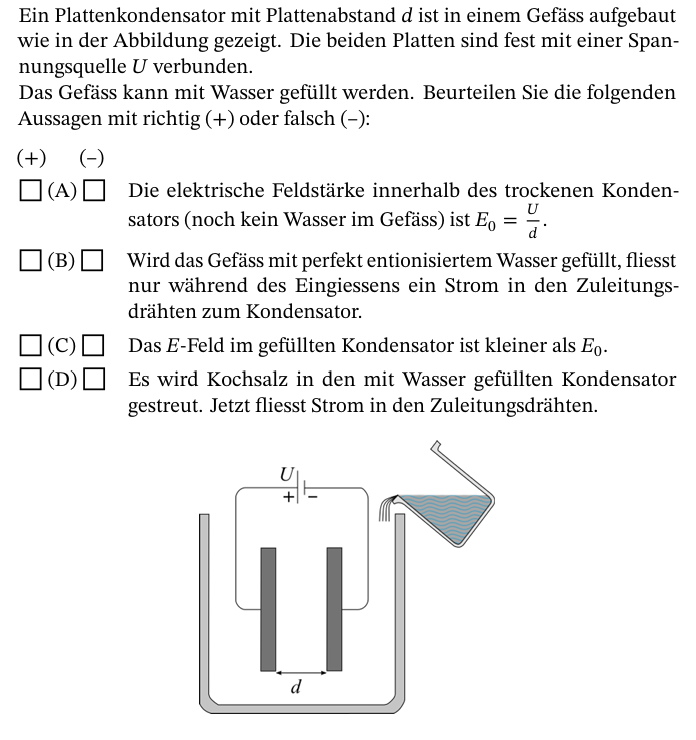
\includegraphics[width=9cm]{Bilder/Kondensator_Wasser_Aufgabe.png}
\end{center}
\begin{solution}
\textbf{(A) Richtig:} $U$ und $d$ sind unverändert, also gilt weiterhin $E_0=U/d$.

\textbf{(B) Richtig:} Entionisiertes Wasser enthält (fast) keine freien Ionen und leitet deshalb nicht -- es wirkt nur als Dielektrikum. Während des Eingiessens steigt der Wasserspiegel zwischen den Platten und damit die Kapazität $C$; da die Batterie $U$ konstant hält, muss dabei Ladung nachfliessen (Ladestrom). Sobald das Gefäss gefüllt ist, ändert sich $C$ nicht mehr, und der Strom hört auf.

\textbf{(C) Falsch:} Die Batterie bleibt angeschlossen und hält $U$ konstant, und $d$ bleibt gleich. Da $E=U/d$, bleibt das Feld unverändert gleich $E_0$ -- es wird \emph{nicht} kleiner. (Das wäre nur der Fall, wenn der Kondensator von der Batterie getrennt wäre und stattdessen $Q$ konstant bliebe.)

\textbf{(D) Richtig:} Kochsalz macht das Wasser zu einem Elektrolyten mit freien Ionen -- es leitet jetzt selbst Strom. Zwischen den Platten fliesst deshalb dauerhaft ein Strom, solange die Batterie angeschlossen bleibt.
\end{solution}
\end{taskbox}

\begin{taskbox}[Aufgabe 9: Abstand nach dem Trennen verändern]
\question[3] Betrachte die Abbildung und beantworte die Frage.
\begin{center}
  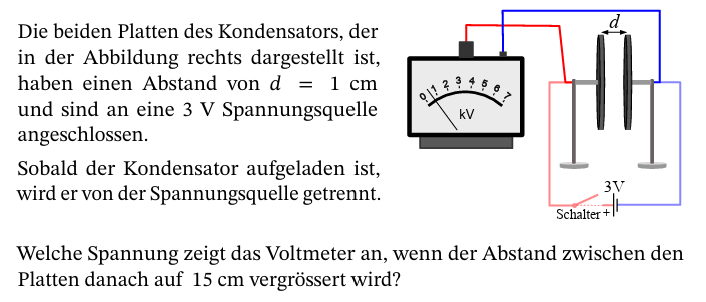
\includegraphics[width=9cm]{Bilder/Kondensator_aufladen_Aufgabe.png}
\end{center}
\Antwortraum{3}
\begin{solution}
Nach dem Trennen bleibt die Ladung $Q$ konstant. Mit $C=\varepsilon_0\cdot A/d$ gilt $C\sim\frac{1}{d}$, also wird die Kapazität beim Vergrössern von $d$ von \SI{1}{\centi\meter} auf \SI{15}{\centi\meter} (Faktor 15) um denselben Faktor kleiner:
\[
  C_2=\frac{C_1}{15}.
\]
Aus $Q=C\cdot U$ konstant folgt:
\[
  C_1\cdot U_1 = C_2\cdot U_2 = \frac{C_1}{15}\cdot U_2 \quad\Longrightarrow\quad U_2 = 15\cdot U_1 = 15\cdot\SI{3}{\volt} = \SI{45}{\volt}.
\]
Das Voltmeter zeigt \SI{45}{\volt} an.
\end{solution}
\end{taskbox}

\end{questions}

\end{document}
